\documentclass[11pt]{article}

\usepackage{lscape,color}
\usepackage{graphicx}

\topmargin -0.75truein
\oddsidemargin -0.4truein
\textheight 9.25truein
\textwidth 6.7truein
\hbadness=10001
\hfuzz=200pt


\begin{document}
%\input dspace12.tex
%\input pstricks.tex
%\input psfig
\newcommand{\be}{\begin{enumerate}}
\newcommand{\ee}{\end{enumerate}}
\newcommand{\bc}{\begin{center}}
\newcommand{\ec}{\end{center}}
\newcommand{\bi}{\begin{itemize}}
\newcommand{\ei}{\end{itemize}}
\newcommand{\bd}{\begin{description}}
\newcommand{\ed}{\end{description}}
\newcommand{\bt}{\begin{tabbing}}
\newcommand{\et}{\end{tabbing}}
\newcommand{\eg}{{\it e.g.~}}
\newcommand{\ie}{{\it i.e.~}}
\newcommand{\ul}{\underline}
\newcommand{\axaf}{{\em AXAF}}

\def\la{\hbox{\rlap{$<$}\lower0.5ex\hbox{$\sim$}\ }}


\large
%\vspace*{-0.5in}
\centerline {\bf 4.30\_V2.3 TURN ON DEA B  }
\vspace{0.25in}

\normalsize
\noindent{\it Last Revised: August 8, 2018}\\
\noindent{\bf Filename: deab\_on} \\


\noindent {\bf BRIEF FUNCTIONAL DESCRIPTION:} \\
\normalsize
This is an ``atomic'' procedure which  powers up the B side of the DEA.
It should be safe to execute under any condition except a spacecraft
power or thermal emergency.

\noindent The sequence of actions for this procedure will be:
\be
\item Verify that DEA A is powered off and disabled (see Constraints/Cautions, below)
\vspace{-0.10in}
\item Verify that DEA B is receiving power from the spacecraft
\vspace{-0.10in}
\item Enable and turn on DEA power supply side B
\vspace{-0.10in}
\item Verify that DEA A is still powered off
\ee

\vspace{0.15in}
\normalsize
\noindent {\bf ASSUMED INSTRUMENT STATE:}
\normalsize
\be
\item The PSMC is receiving power from the spacecraft
\vspace{-0.10in}
\item DEA A is powered off
\ee

\vspace{0.15in}
\normalsize
\noindent {\bf SPECIAL INITIAL CONDITIONS:} \\
\normalsize
%The environment must be clean enough to allow opening of the valve. \\
%Assumes that \axaf\/ ISIM RCTU is powered on and in telemetry format 6. \\

%\vspace{0.25in}
\normalsize
\noindent {\bf OPERATIONAL CONSTRAINTS/CAUTIONS:} \\
\normalsize
In normal operations, only one side of the DEA should be powered on
(a) to prevent conflict for control of the focal plane temperature controller,
(b) to avoid excess current draw from the spacecraft, and (c) to avoid over-heating
within the PSMC.

The DEA power status is normally indicated by the values of the 1DEPSA and
1DEPSB flags, which should not both be 1 simultaneously.
However, if neither side of the DPA is receiving power
({\it i.e.}, if 1DPP0AVO and 1DPP0BVO are simultaneously reading $0.0 \pm 0.5$ V),
the DEA flag values will be unreliable and the DEA voltage
channels (1DEP[0123][AB]VO) should instead be used to determine which
sides of the DEA are powered).

The DEA input current monitors (1DEIC[AB]CU) are noisy.
To give an indication of what variation may be expected, figures 1 and 2
show the behavior of the A-side DEA current with a ten-sample running
average for two situations in which all video boards were powered down.
Note that when either side of the DEA is unpowered, the corresponding current monitor,
1DEICBCU for side B, or 1DEICACU for side A, will be unreliable.
They will read $16-18$~A when unpowered, as of Telemetry Database TDB v14.
This is expected and not a problem.

After successful execution, {\em the FP temperature control will be unregulated,
and DEA interface A/D will be in low-resolution mode.}

\vspace{0.15in}
\normalsize
\noindent {\bf REFERENCES:} \\
\normalsize

\normalsize
\noindent {\bf CHANGE HISTORY:} \\
\normalsize

{\bf V1.0}
\begin{itemize}
\item Initial version, based on deaa\_on.
\end{itemize}

{\bf V1.1}
\begin{itemize}
\item Minor edits, for ACIS team review
\end{itemize}

{\bf V1.2}
\begin{itemize}
\item Added caution about using both DEA power supplies at once. 
For ACIS team review.
\end{itemize}

{\bf V1.3}
\begin{itemize}
\item Extra DEA-A off checks
\end{itemize}

{\bf V2.0}
\begin{itemize}
\item For FOT review
\end{itemize}

{\bf V2.1}
\begin{itemize}
\item Corrected expected voltages; added +28V input checks.
\end{itemize}

{\bf V2.2}
\begin{itemize}
\item Removed input current check; added warning to text.
\end{itemize}

{\bf V2.3}
\begin{itemize}
\item Added a new step to verify that DEA B is receiving power from the spacecraft.
\end{itemize}

\begin{landscape}
\begin{figure}
\begin{center}
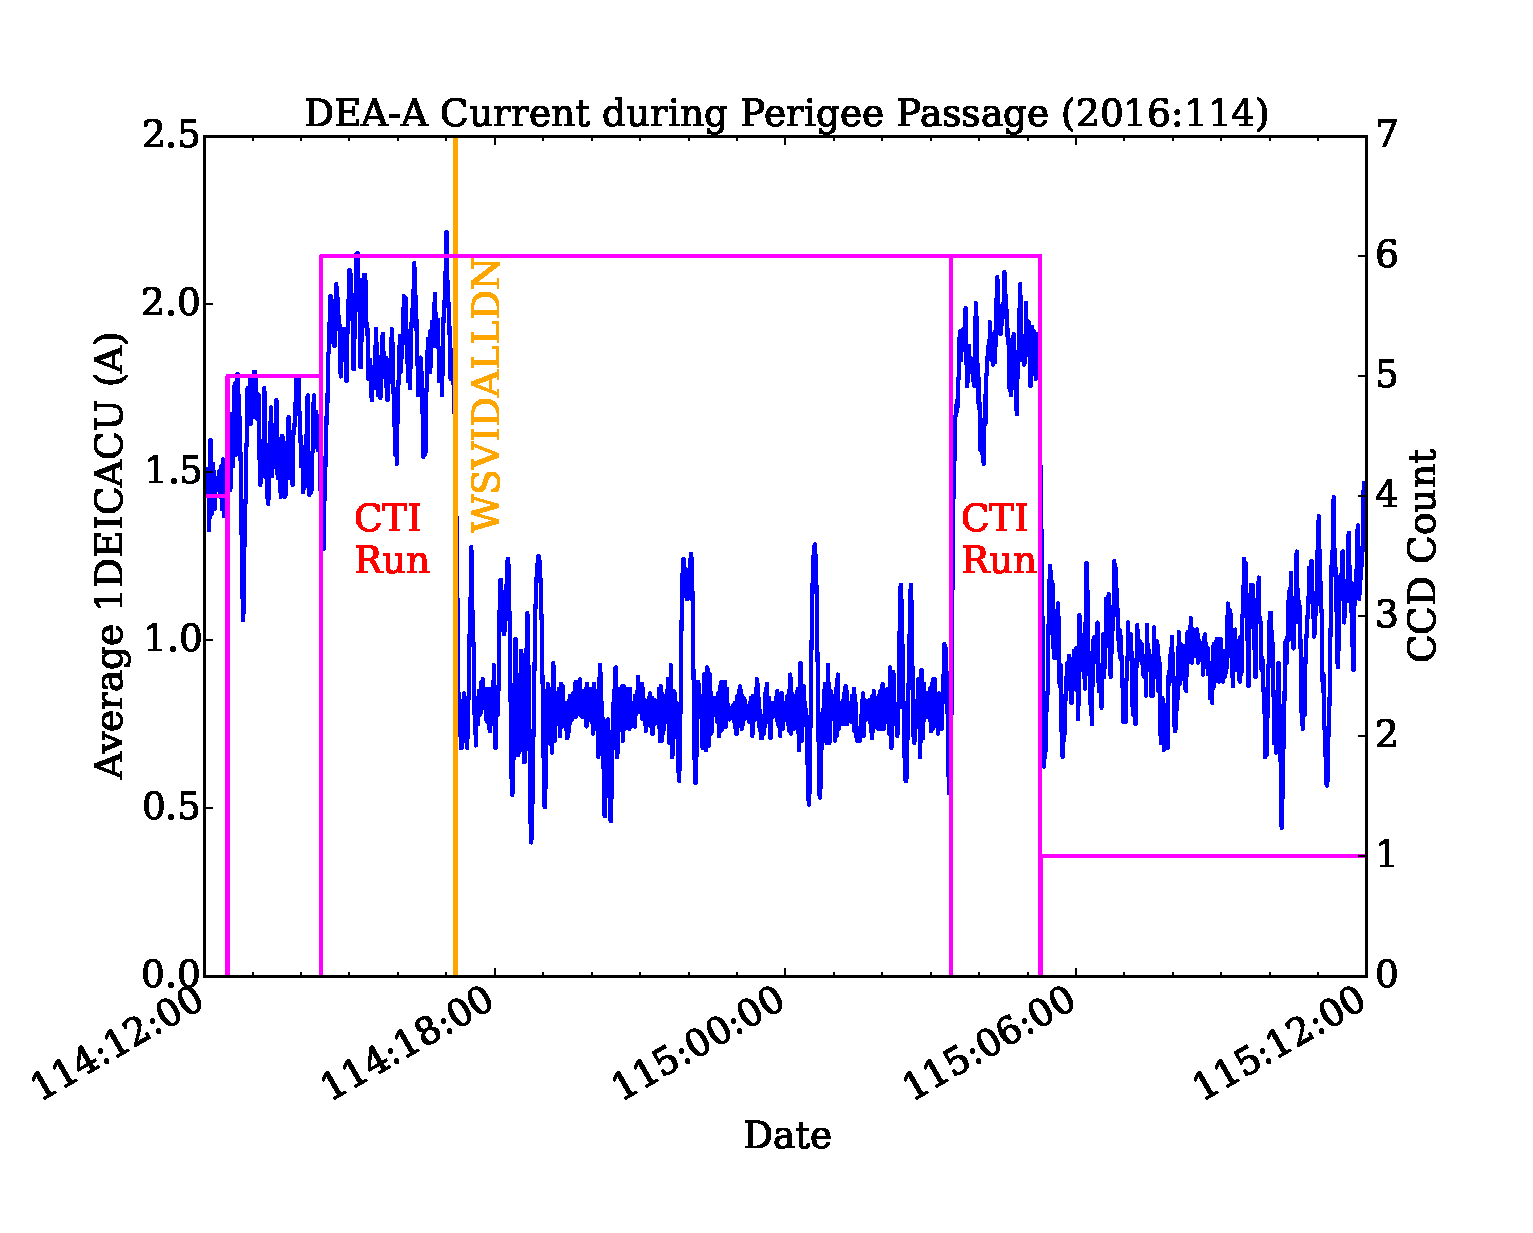
\includegraphics[width=1.2\textwidth]{deaa_on_fig1.eps}
\caption{Ten-sample running average behavior of 1DEICACU during a perigee passage.
All video boards are powered off after the issuing of the WSVIDALLDN command,
which is marked by the orange line in the plot.}
\end{center}
\end{figure}
\end{landscape}

\begin{landscape}
\begin{figure}
\begin{center}
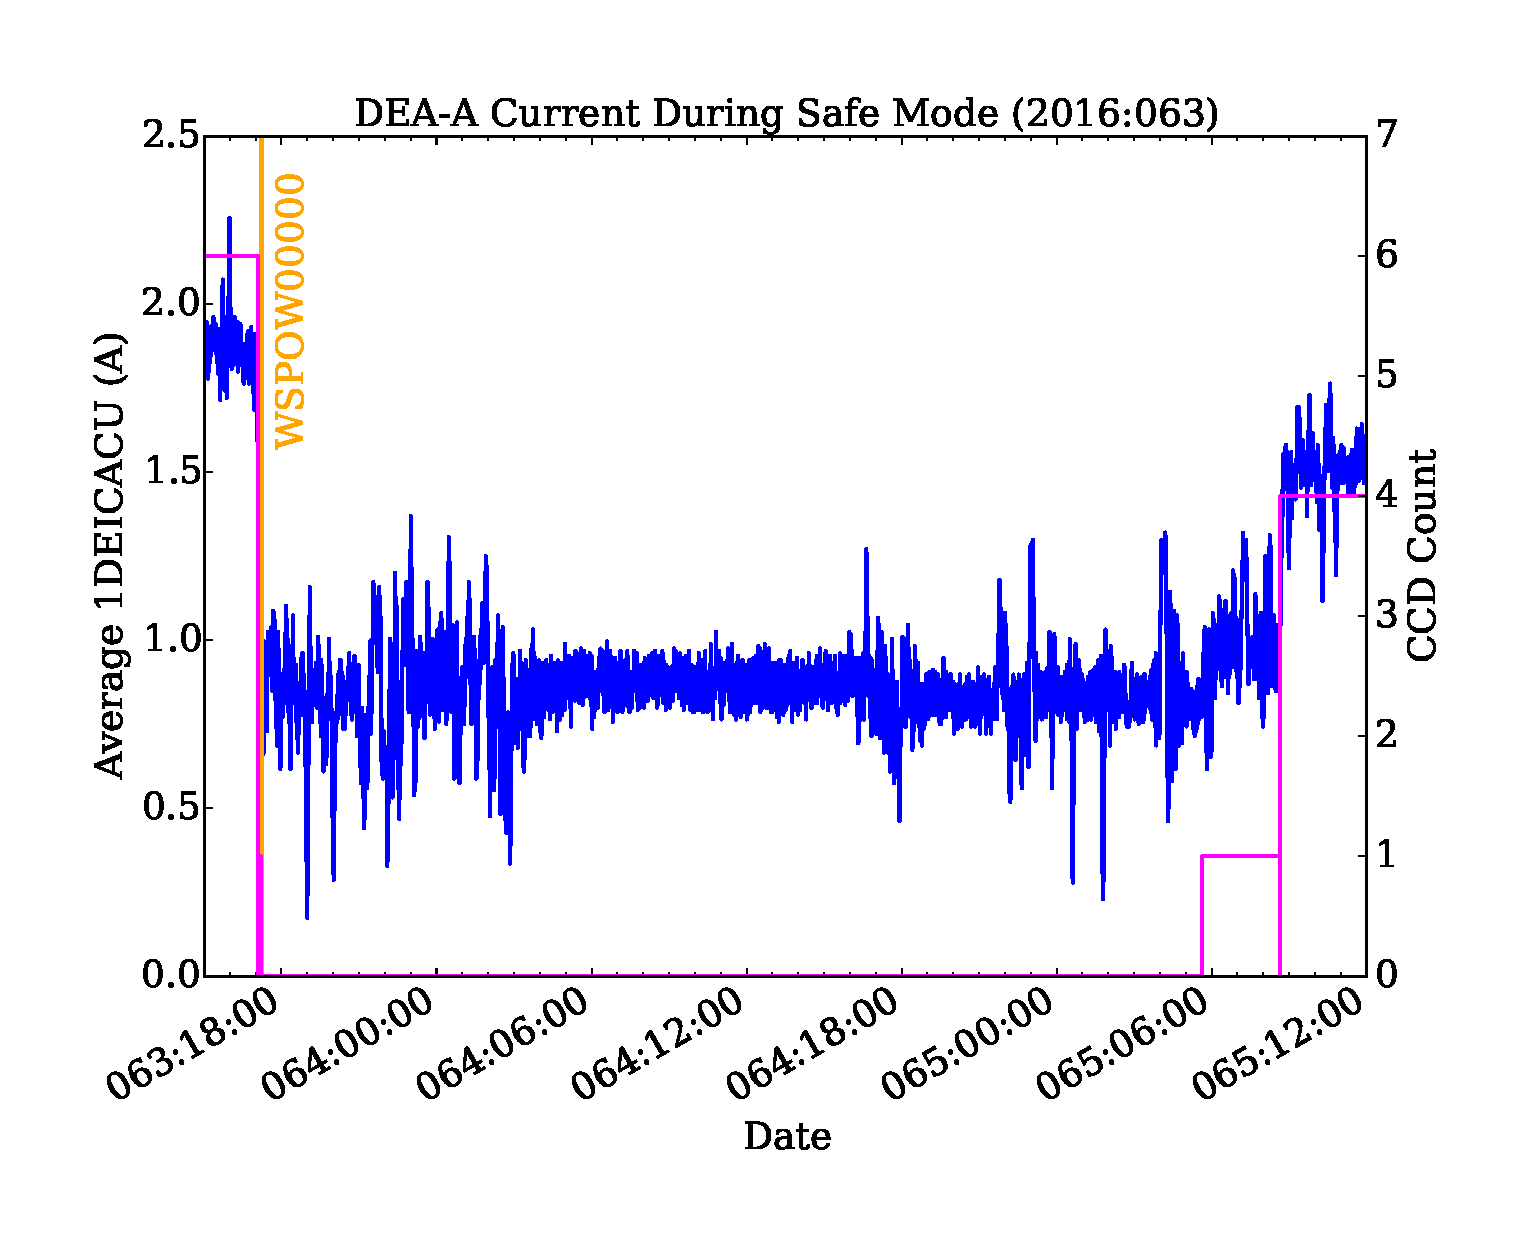
\includegraphics[width=1.2\textwidth]{deaa_on_fig2.eps}
\caption{Ten-sample running average behavior of 1DEICACU during a safe mode.
All video boards are powered off after the issuing of the WSPOW00000 command,
which is marked by the orange line in the plot.}
\end{center}
\end{figure}
\end{landscape}

\newpage\
\vspace{0.4\textheight}
\bc This page is intentionally blank \ec

\newcommand{\tablecaptiontext}{TURN ON DEA B (realtime version)}
\documentclass[11pt]{article}

\usepackage{lscape,color}
\usepackage{graphicx}

\topmargin -0.75truein
\oddsidemargin -0.4truein
\textheight 9.25truein
\textwidth 6.7truein
\hbadness=10001
\hfuzz=200pt


\begin{document}
%\input dspace12.tex
%\input pstricks.tex
%\input psfig
\newcommand{\be}{\begin{enumerate}}
\newcommand{\ee}{\end{enumerate}}
\newcommand{\bc}{\begin{center}}
\newcommand{\ec}{\end{center}}
\newcommand{\bi}{\begin{itemize}}
\newcommand{\ei}{\end{itemize}}
\newcommand{\bd}{\begin{description}}
\newcommand{\ed}{\end{description}}
\newcommand{\bt}{\begin{tabbing}}
\newcommand{\et}{\end{tabbing}}
\newcommand{\eg}{{\it e.g.~}}
\newcommand{\ie}{{\it i.e.~}}
\newcommand{\ul}{\underline}
\newcommand{\axaf}{{\em AXAF}}

\def\la{\hbox{\rlap{$<$}\lower0.5ex\hbox{$\sim$}\ }}


\large
%\vspace*{-0.5in}
\centerline {\bf 4.30\_V2.2 TURN ON DEA B  }
\vspace{0.25in}

\normalsize
\noindent{\it Last Revised: May 25, 2017}\\
\noindent{\bf Filename: deab\_on} \\


\noindent {\bf BRIEF FUNCTIONAL DESCRIPTION:} \\
\normalsize
This is an ``atomic'' procedure which  powers up the B side of the DEA.
It should be safe to execute under any condition except a spacecraft
power or thermal emergency.

\noindent The sequence of actions for this procedure will be:
\be
\item Verify that DEA A is powered off and disabled (see Constraints/Cautions, below)
\vspace{-0.10in}
\item Enable and turn on DEA power supply side B
\vspace{-0.10in}
\item Verify that DEA A is still powered off
\ee

\vspace{0.15in}
\normalsize
\noindent {\bf ASSUMED INSTRUMENT STATE:}
\normalsize
\be
\item The PSMC is receiving power from the spacecraft
\vspace{-0.10in}
\item DEA A is powered off
\ee

\vspace{0.15in}
\normalsize
\noindent {\bf SPECIAL INITIAL CONDITIONS:} \\
\normalsize
%The environment must be clean enough to allow opening of the valve. \\
%Assumes that \axaf\/ ISIM RCTU is powered on and in telemetry format 6. \\

%\vspace{0.25in}
\normalsize
\noindent {\bf OPERATIONAL CONSTRAINTS/CAUTIONS:} \\
\normalsize
In normal operations, only one side of the DEA should be powered on
(a) to prevent conflict for control of the focal plane temperature controller,
(b) to avoid excess current draw from the spacecraft, and (c) to avoid over-heating
within the PSMC.

The DEA power status is normally indicated by the values of the 1DEPSA and
1DEPSB flags, which should not both be 1 simultaneously.
However, if neither side of the DPA is receiving power
({\it i.e.}, if 1DPP0AVO and 1DPP0BVO are simultaneously reading $0.0 \pm 0.5$ V),
the DEA flag values will be unreliable and the DEA voltage
channels (1DEP[0123][AB]VO) should instead be used to determine which
sides of the DEA are powered).

The DEA input current monitors (1DEIC[AB]CU) are noisy.
To give an indication of what variation may be expected, figures 1 and 2
show the behavior of the A-side DEA current with a ten-sample running
average for two situations in which all video boards were powered down.
Note that when either side of the DEA is unpowered, the corresponding current monitor,
1DEICBCU for side B, or 1DEICACU for side A, will be unreliable.
They will read $16-18$~A when unpowered, as of Telemetry Database TDB v14.
This is expected and not a problem.

After successful execution, {\em the FP temperature control will be unregulated,
and DEA interface A/D will be in low-resolution mode.}

\vspace{0.15in}
\normalsize
\noindent {\bf REFERENCES:} \\
\normalsize

\normalsize
\noindent {\bf CHANGE HISTORY:} \\
\normalsize

{\bf V1.0}
\begin{itemize}
\item Initial version, based on deaa\_on.
\end{itemize}

{\bf V1.1}
\begin{itemize}
\item Minor edits, for ACIS team review
\end{itemize}

{\bf V1.2}
\begin{itemize}
\item Added caution about using both DEA power supplies at once. 
For ACIS team review.
\end{itemize}

{\bf V1.3}
\begin{itemize}
\item Extra DEA-A off checks
\end{itemize}

{\bf V2.0}
\begin{itemize}
\item For FOT review
\end{itemize}

{\bf V2.1}
\begin{itemize}
\item Corrected expected voltages; added +28V input checks.
\end{itemize}

{\bf V2.2}
\begin{itemize}
\item Removed input current check; added warning to text.
\end{itemize}

\begin{landscape}
\begin{figure}
\begin{center}
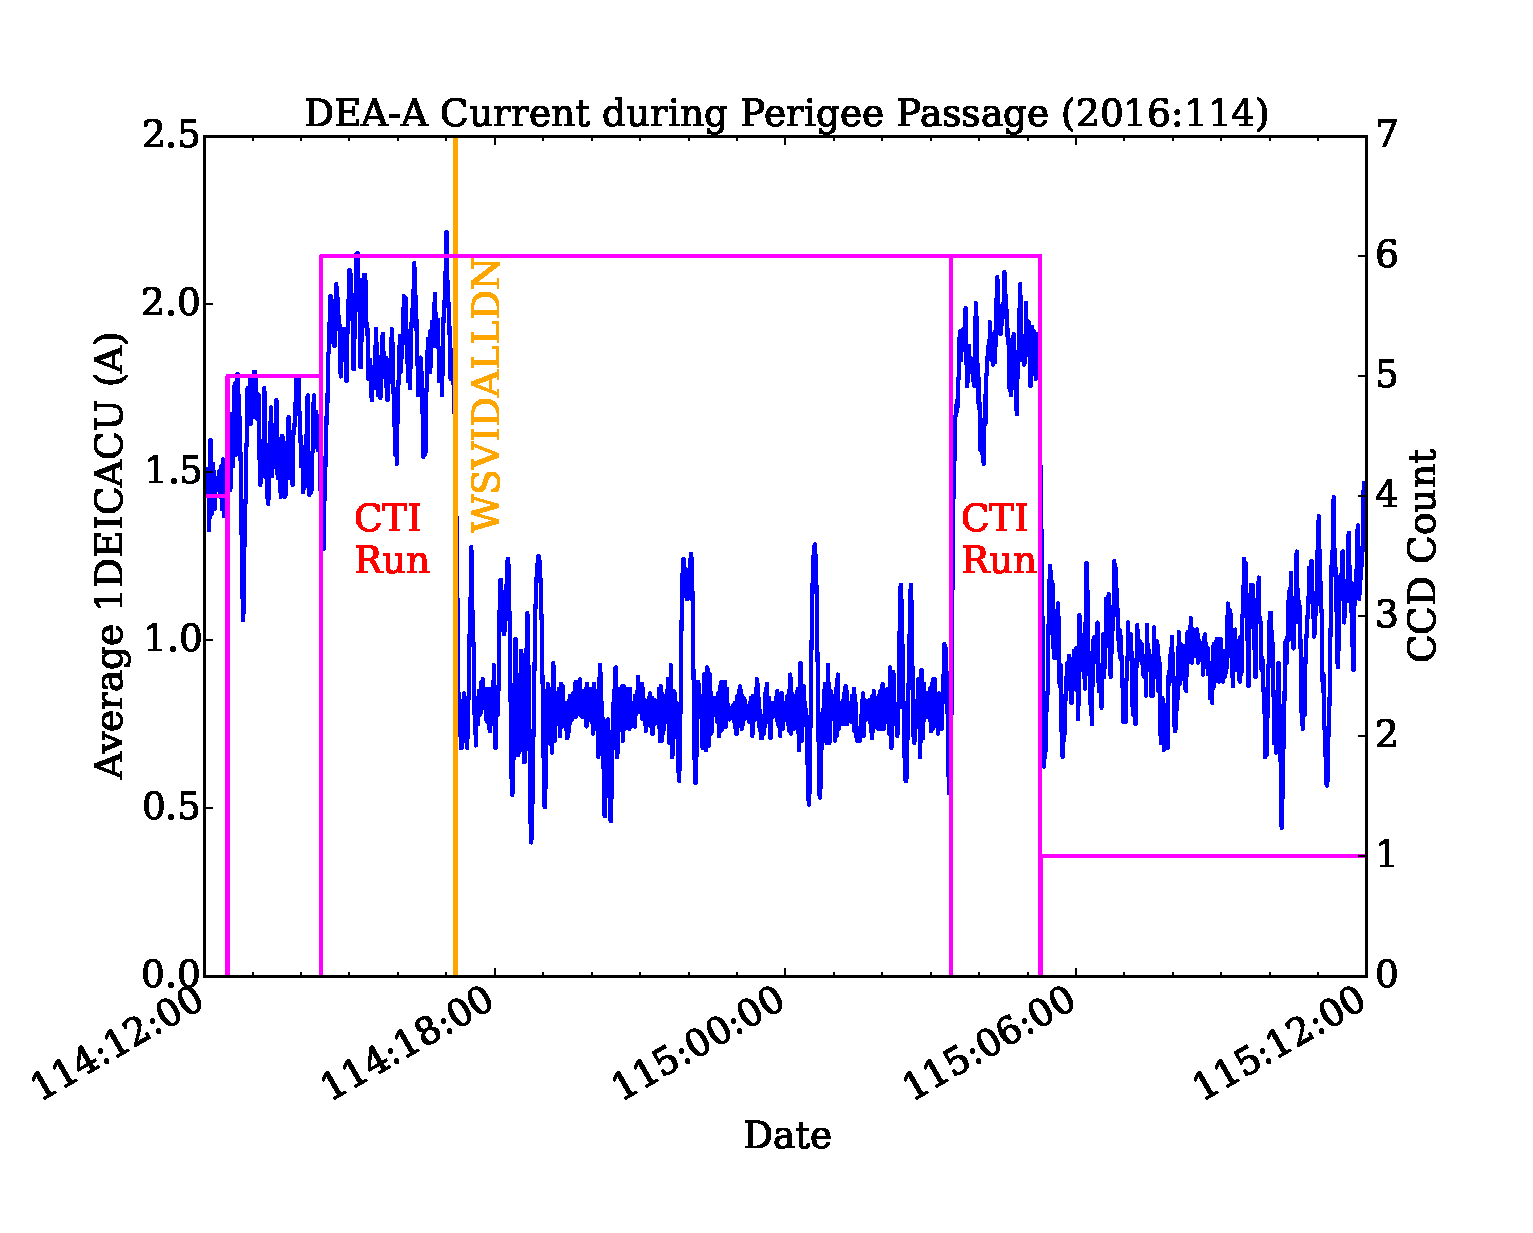
\includegraphics[width=1.2\textwidth]{deaa_on_fig1.eps}
\caption{Ten-sample running average behavior of 1DEICACU during a perigee passage.
All video boards are powered off after the issuing of the WSVIDALLDN command,
which is marked by the orange line in the plot.}
\end{center}
\end{figure}
\end{landscape}

\begin{landscape}
\begin{figure}
\begin{center}
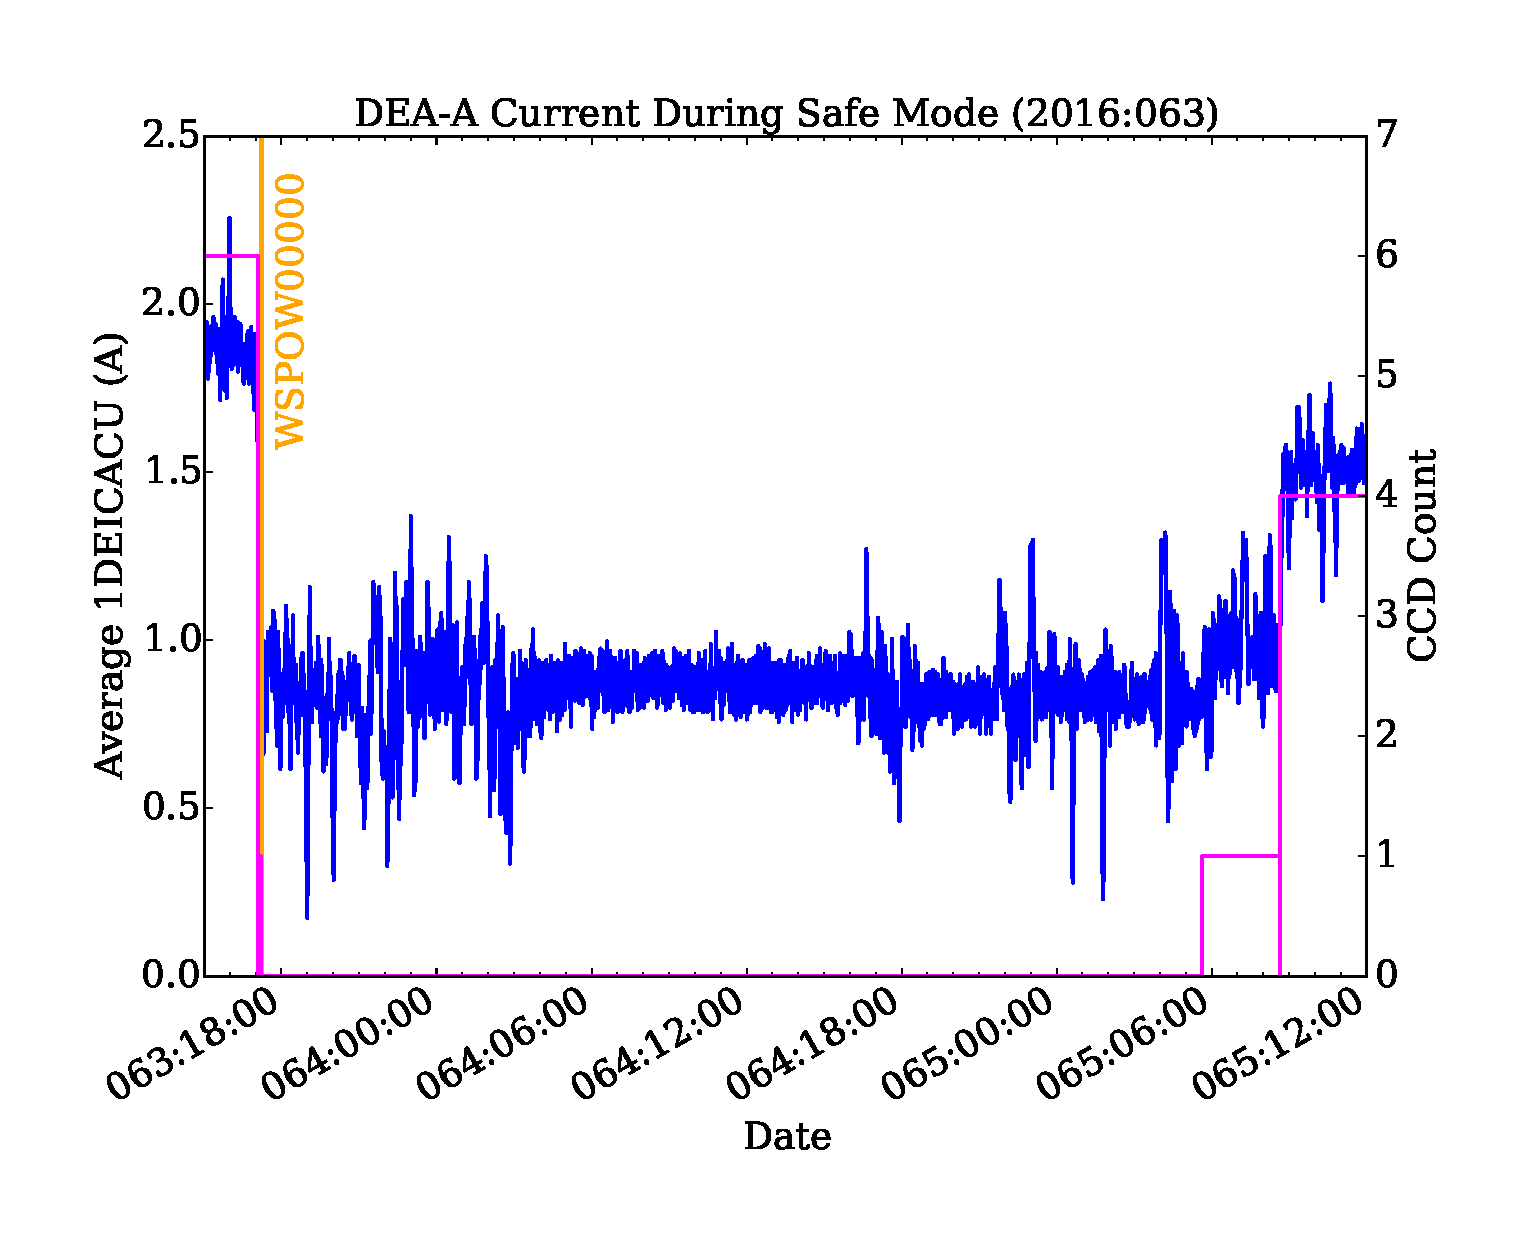
\includegraphics[width=1.2\textwidth]{deaa_on_fig2.eps}
\caption{Ten-sample running average behavior of 1DEICACU during a safe mode.
All video boards are powered off after the issuing of the WSPOW00000 command,
which is marked by the orange line in the plot.}
\end{center}
\end{figure}
\end{landscape}

\newpage\
\vspace{0.4\textheight}
\bc This page is intentionally blank \ec

\newcommand{\tablecaptiontext}{TURN ON DEA B (realtime version)}
\documentclass[11pt]{article}

\usepackage{lscape,color}
\usepackage{graphicx}

\topmargin -0.75truein
\oddsidemargin -0.4truein
\textheight 9.25truein
\textwidth 6.7truein
\hbadness=10001
\hfuzz=200pt


\begin{document}
%\input dspace12.tex
%\input pstricks.tex
%\input psfig
\newcommand{\be}{\begin{enumerate}}
\newcommand{\ee}{\end{enumerate}}
\newcommand{\bc}{\begin{center}}
\newcommand{\ec}{\end{center}}
\newcommand{\bi}{\begin{itemize}}
\newcommand{\ei}{\end{itemize}}
\newcommand{\bd}{\begin{description}}
\newcommand{\ed}{\end{description}}
\newcommand{\bt}{\begin{tabbing}}
\newcommand{\et}{\end{tabbing}}
\newcommand{\eg}{{\it e.g.~}}
\newcommand{\ie}{{\it i.e.~}}
\newcommand{\ul}{\underline}
\newcommand{\axaf}{{\em AXAF}}

\def\la{\hbox{\rlap{$<$}\lower0.5ex\hbox{$\sim$}\ }}


\large
%\vspace*{-0.5in}
\centerline {\bf 4.30\_V2.2 TURN ON DEA B  }
\vspace{0.25in}

\normalsize
\noindent{\it Last Revised: May 25, 2017}\\
\noindent{\bf Filename: deab\_on} \\


\noindent {\bf BRIEF FUNCTIONAL DESCRIPTION:} \\
\normalsize
This is an ``atomic'' procedure which  powers up the B side of the DEA.
It should be safe to execute under any condition except a spacecraft
power or thermal emergency.

\noindent The sequence of actions for this procedure will be:
\be
\item Verify that DEA A is powered off and disabled (see Constraints/Cautions, below)
\vspace{-0.10in}
\item Enable and turn on DEA power supply side B
\vspace{-0.10in}
\item Verify that DEA A is still powered off
\ee

\vspace{0.15in}
\normalsize
\noindent {\bf ASSUMED INSTRUMENT STATE:}
\normalsize
\be
\item The PSMC is receiving power from the spacecraft
\vspace{-0.10in}
\item DEA A is powered off
\ee

\vspace{0.15in}
\normalsize
\noindent {\bf SPECIAL INITIAL CONDITIONS:} \\
\normalsize
%The environment must be clean enough to allow opening of the valve. \\
%Assumes that \axaf\/ ISIM RCTU is powered on and in telemetry format 6. \\

%\vspace{0.25in}
\normalsize
\noindent {\bf OPERATIONAL CONSTRAINTS/CAUTIONS:} \\
\normalsize
In normal operations, only one side of the DEA should be powered on
(a) to prevent conflict for control of the focal plane temperature controller,
(b) to avoid excess current draw from the spacecraft, and (c) to avoid over-heating
within the PSMC.

The DEA power status is normally indicated by the values of the 1DEPSA and
1DEPSB flags, which should not both be 1 simultaneously.
However, if neither side of the DPA is receiving power
({\it i.e.}, if 1DPP0AVO and 1DPP0BVO are simultaneously reading $0.0 \pm 0.5$ V),
the DEA flag values will be unreliable and the DEA voltage
channels (1DEP[0123][AB]VO) should instead be used to determine which
sides of the DEA are powered).

The DEA input current monitors (1DEIC[AB]CU) are noisy.
To give an indication of what variation may be expected, figures 1 and 2
show the behavior of the A-side DEA current with a ten-sample running
average for two situations in which all video boards were powered down.
Note that when either side of the DEA is unpowered, the corresponding current monitor,
1DEICBCU for side B, or 1DEICACU for side A, will be unreliable.
They will read $16-18$~A when unpowered, as of Telemetry Database TDB v14.
This is expected and not a problem.

After successful execution, {\em the FP temperature control will be unregulated,
and DEA interface A/D will be in low-resolution mode.}

\vspace{0.15in}
\normalsize
\noindent {\bf REFERENCES:} \\
\normalsize

\normalsize
\noindent {\bf CHANGE HISTORY:} \\
\normalsize

{\bf V1.0}
\begin{itemize}
\item Initial version, based on deaa\_on.
\end{itemize}

{\bf V1.1}
\begin{itemize}
\item Minor edits, for ACIS team review
\end{itemize}

{\bf V1.2}
\begin{itemize}
\item Added caution about using both DEA power supplies at once. 
For ACIS team review.
\end{itemize}

{\bf V1.3}
\begin{itemize}
\item Extra DEA-A off checks
\end{itemize}

{\bf V2.0}
\begin{itemize}
\item For FOT review
\end{itemize}

{\bf V2.1}
\begin{itemize}
\item Corrected expected voltages; added +28V input checks.
\end{itemize}

{\bf V2.2}
\begin{itemize}
\item Removed input current check; added warning to text.
\end{itemize}

\begin{landscape}
\begin{figure}
\begin{center}
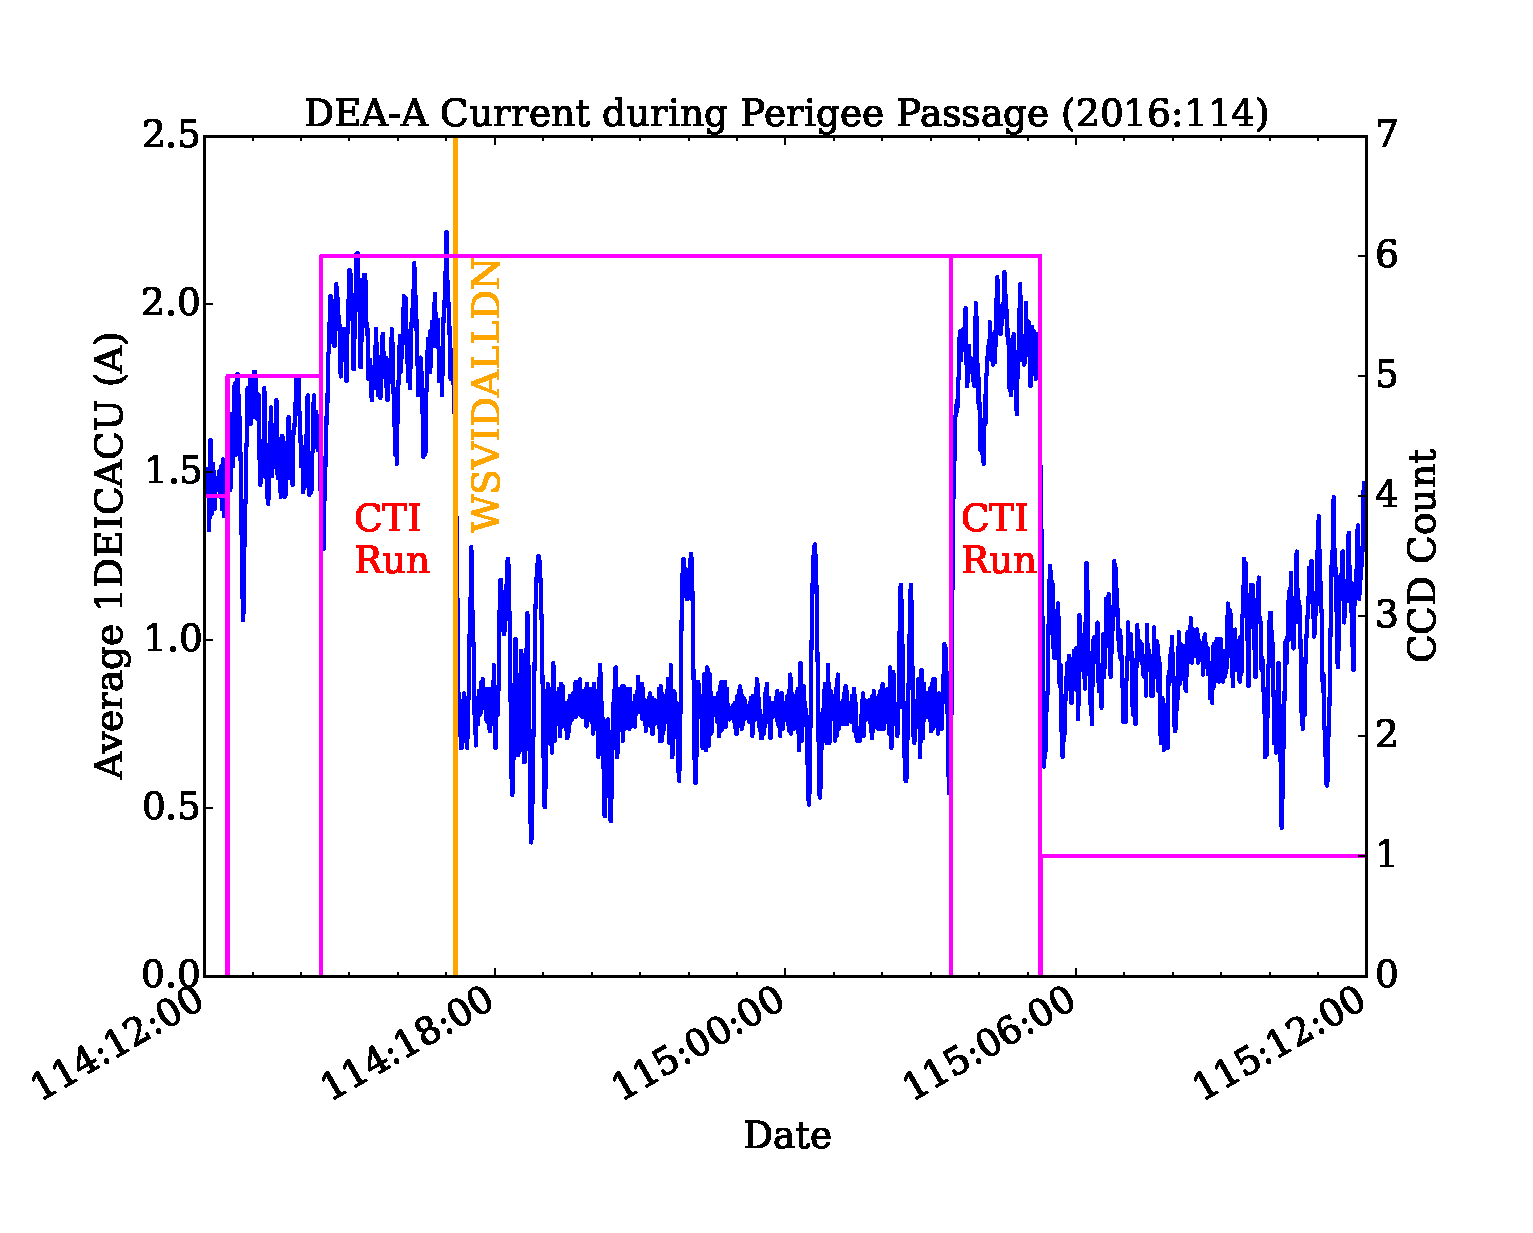
\includegraphics[width=1.2\textwidth]{deaa_on_fig1.eps}
\caption{Ten-sample running average behavior of 1DEICACU during a perigee passage.
All video boards are powered off after the issuing of the WSVIDALLDN command,
which is marked by the orange line in the plot.}
\end{center}
\end{figure}
\end{landscape}

\begin{landscape}
\begin{figure}
\begin{center}
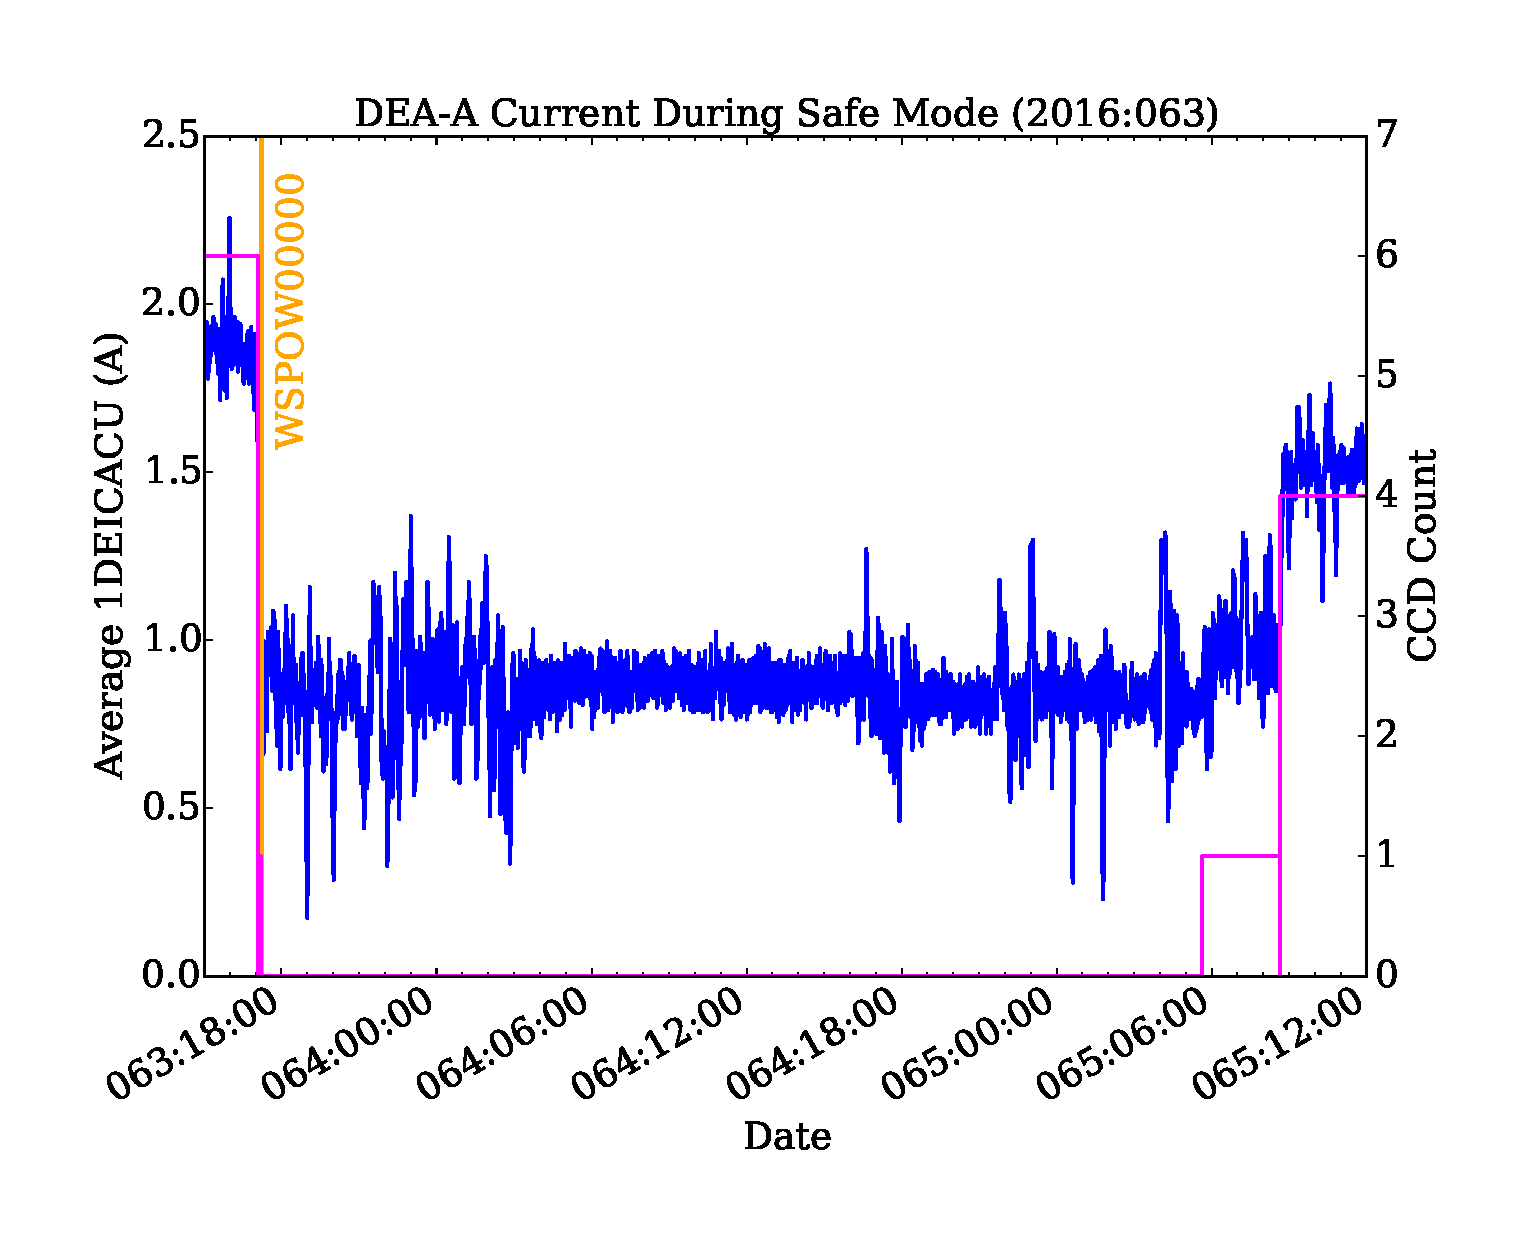
\includegraphics[width=1.2\textwidth]{deaa_on_fig2.eps}
\caption{Ten-sample running average behavior of 1DEICACU during a safe mode.
All video boards are powered off after the issuing of the WSPOW00000 command,
which is marked by the orange line in the plot.}
\end{center}
\end{figure}
\end{landscape}

\newpage\
\vspace{0.4\textheight}
\bc This page is intentionally blank \ec

\newcommand{\tablecaptiontext}{TURN ON DEA B (realtime version)}
\documentclass[11pt]{article}

\usepackage{lscape,color}
\usepackage{graphicx}

\topmargin -0.75truein
\oddsidemargin -0.4truein
\textheight 9.25truein
\textwidth 6.7truein
\hbadness=10001
\hfuzz=200pt


\begin{document}
%\input dspace12.tex
%\input pstricks.tex
%\input psfig
\newcommand{\be}{\begin{enumerate}}
\newcommand{\ee}{\end{enumerate}}
\newcommand{\bc}{\begin{center}}
\newcommand{\ec}{\end{center}}
\newcommand{\bi}{\begin{itemize}}
\newcommand{\ei}{\end{itemize}}
\newcommand{\bd}{\begin{description}}
\newcommand{\ed}{\end{description}}
\newcommand{\bt}{\begin{tabbing}}
\newcommand{\et}{\end{tabbing}}
\newcommand{\eg}{{\it e.g.~}}
\newcommand{\ie}{{\it i.e.~}}
\newcommand{\ul}{\underline}
\newcommand{\axaf}{{\em AXAF}}

\def\la{\hbox{\rlap{$<$}\lower0.5ex\hbox{$\sim$}\ }}


\large
%\vspace*{-0.5in}
\centerline {\bf 4.30\_V2.2 TURN ON DEA B  }
\vspace{0.25in}

\normalsize
\noindent{\it Last Revised: May 25, 2017}\\
\noindent{\bf Filename: deab\_on} \\


\noindent {\bf BRIEF FUNCTIONAL DESCRIPTION:} \\
\normalsize
This is an ``atomic'' procedure which  powers up the B side of the DEA.
It should be safe to execute under any condition except a spacecraft
power or thermal emergency.

\noindent The sequence of actions for this procedure will be:
\be
\item Verify that DEA A is powered off and disabled (see Constraints/Cautions, below)
\vspace{-0.10in}
\item Enable and turn on DEA power supply side B
\vspace{-0.10in}
\item Verify that DEA A is still powered off
\ee

\vspace{0.15in}
\normalsize
\noindent {\bf ASSUMED INSTRUMENT STATE:}
\normalsize
\be
\item The PSMC is receiving power from the spacecraft
\vspace{-0.10in}
\item DEA A is powered off
\ee

\vspace{0.15in}
\normalsize
\noindent {\bf SPECIAL INITIAL CONDITIONS:} \\
\normalsize
%The environment must be clean enough to allow opening of the valve. \\
%Assumes that \axaf\/ ISIM RCTU is powered on and in telemetry format 6. \\

%\vspace{0.25in}
\normalsize
\noindent {\bf OPERATIONAL CONSTRAINTS/CAUTIONS:} \\
\normalsize
In normal operations, only one side of the DEA should be powered on
(a) to prevent conflict for control of the focal plane temperature controller,
(b) to avoid excess current draw from the spacecraft, and (c) to avoid over-heating
within the PSMC.

The DEA power status is normally indicated by the values of the 1DEPSA and
1DEPSB flags, which should not both be 1 simultaneously.
However, if neither side of the DPA is receiving power
({\it i.e.}, if 1DPP0AVO and 1DPP0BVO are simultaneously reading $0.0 \pm 0.5$ V),
the DEA flag values will be unreliable and the DEA voltage
channels (1DEP[0123][AB]VO) should instead be used to determine which
sides of the DEA are powered).

The DEA input current monitors (1DEIC[AB]CU) are noisy.
To give an indication of what variation may be expected, figures 1 and 2
show the behavior of the A-side DEA current with a ten-sample running
average for two situations in which all video boards were powered down.
Note that when either side of the DEA is unpowered, the corresponding current monitor,
1DEICBCU for side B, or 1DEICACU for side A, will be unreliable.
They will read $16-18$~A when unpowered, as of Telemetry Database TDB v14.
This is expected and not a problem.

After successful execution, {\em the FP temperature control will be unregulated,
and DEA interface A/D will be in low-resolution mode.}

\vspace{0.15in}
\normalsize
\noindent {\bf REFERENCES:} \\
\normalsize

\normalsize
\noindent {\bf CHANGE HISTORY:} \\
\normalsize

{\bf V1.0}
\begin{itemize}
\item Initial version, based on deaa\_on.
\end{itemize}

{\bf V1.1}
\begin{itemize}
\item Minor edits, for ACIS team review
\end{itemize}

{\bf V1.2}
\begin{itemize}
\item Added caution about using both DEA power supplies at once. 
For ACIS team review.
\end{itemize}

{\bf V1.3}
\begin{itemize}
\item Extra DEA-A off checks
\end{itemize}

{\bf V2.0}
\begin{itemize}
\item For FOT review
\end{itemize}

{\bf V2.1}
\begin{itemize}
\item Corrected expected voltages; added +28V input checks.
\end{itemize}

{\bf V2.2}
\begin{itemize}
\item Removed input current check; added warning to text.
\end{itemize}

\begin{landscape}
\begin{figure}
\begin{center}
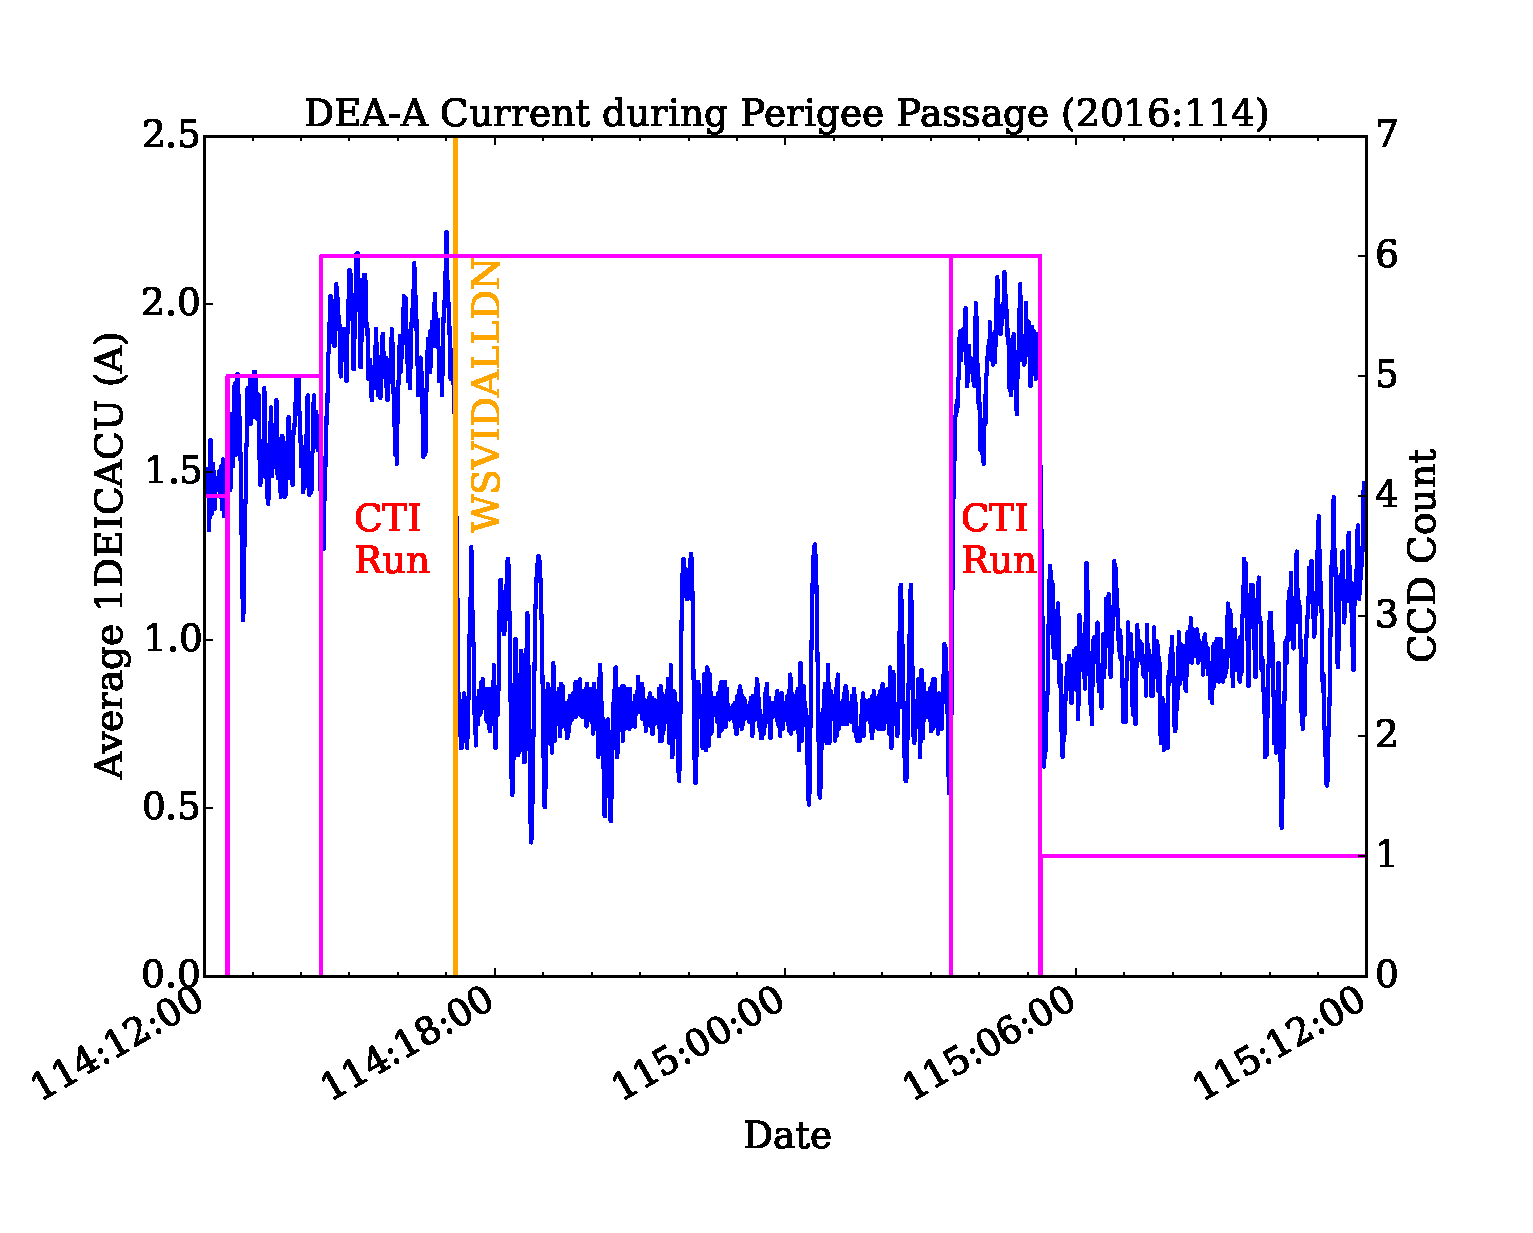
\includegraphics[width=1.2\textwidth]{deaa_on_fig1.eps}
\caption{Ten-sample running average behavior of 1DEICACU during a perigee passage.
All video boards are powered off after the issuing of the WSVIDALLDN command,
which is marked by the orange line in the plot.}
\end{center}
\end{figure}
\end{landscape}

\begin{landscape}
\begin{figure}
\begin{center}
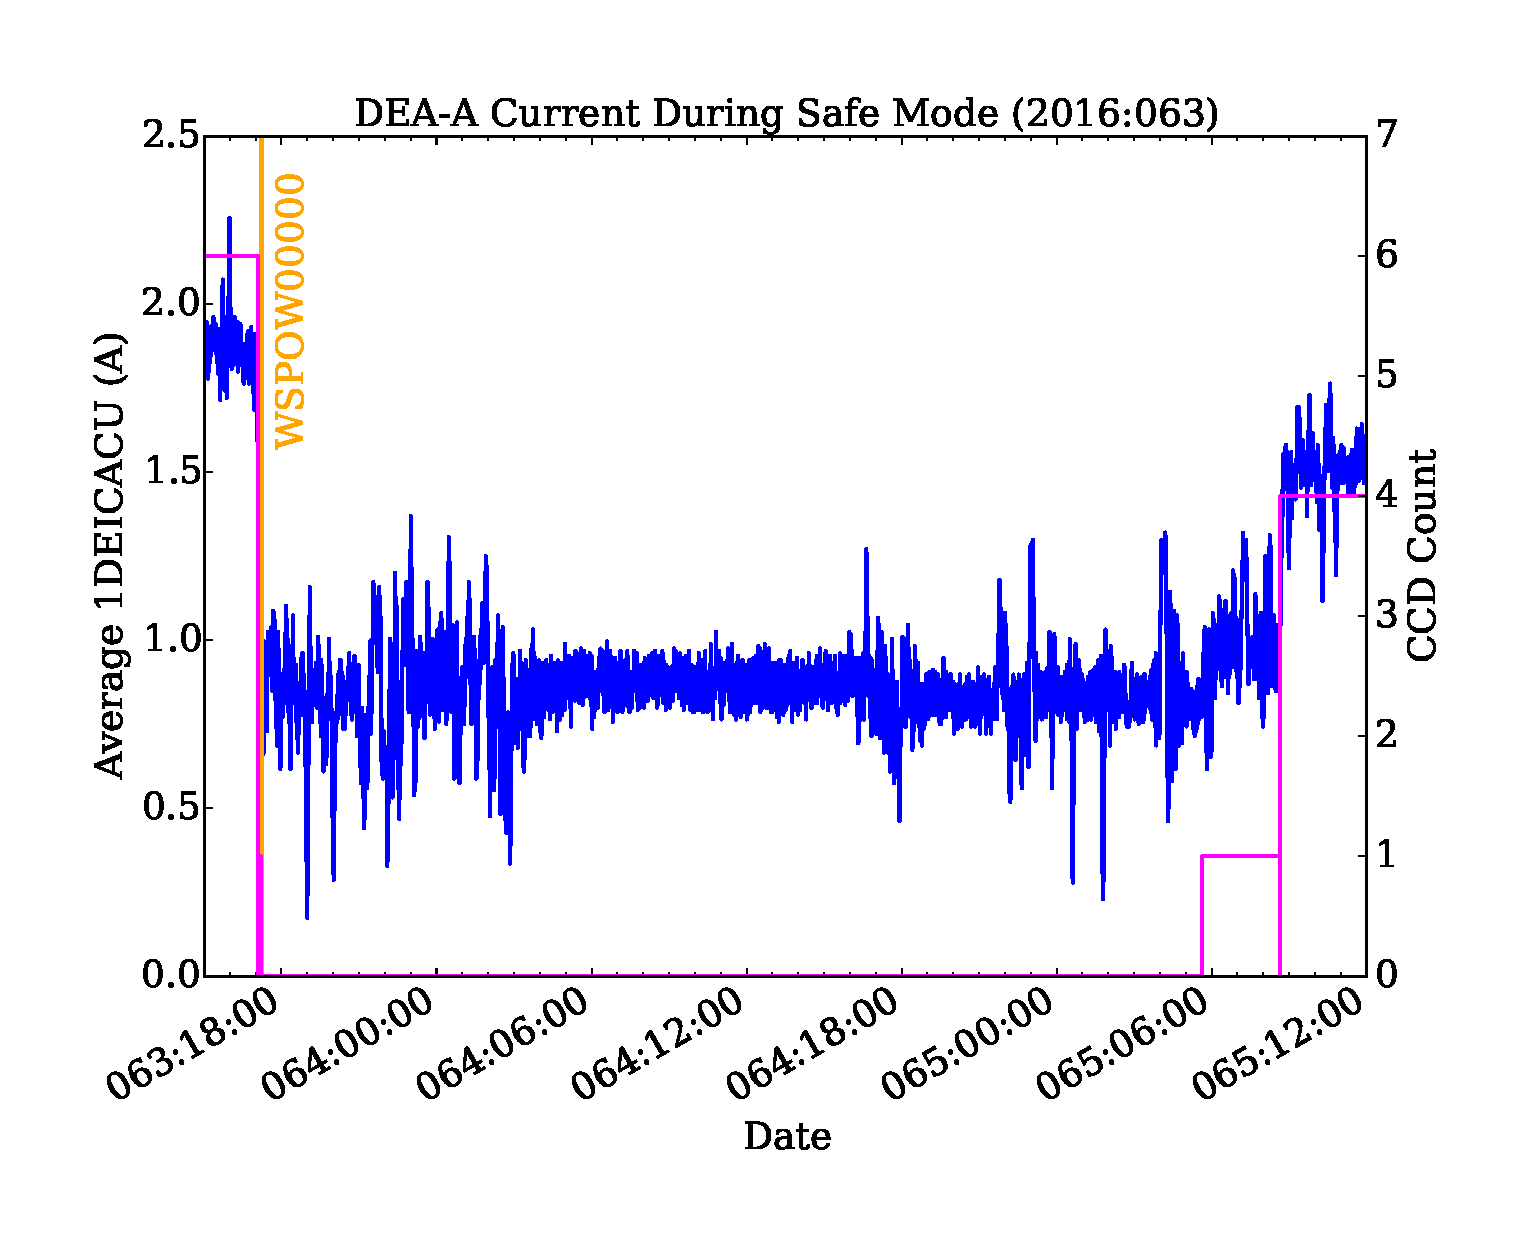
\includegraphics[width=1.2\textwidth]{deaa_on_fig2.eps}
\caption{Ten-sample running average behavior of 1DEICACU during a safe mode.
All video boards are powered off after the issuing of the WSPOW00000 command,
which is marked by the orange line in the plot.}
\end{center}
\end{figure}
\end{landscape}

\newpage\
\vspace{0.4\textheight}
\bc This page is intentionally blank \ec

\newcommand{\tablecaptiontext}{TURN ON DEA B (realtime version)}
\input{deab_on.tab}

\end{document}


\end{document}


\end{document}


\end{document}
